% Template:     Informe LaTeX
% Documento:    Archivo de ejemplo
% Versión:      8.4.4 (02/12/2025)
% Codificación: UTF-8
%
% Autor: Pablo Pizarro R.
%        pablo@ppizarror.com
%
% Manual template: [https://latex.ppizarror.com/informe]
% Licencia MIT:    [https://opensource.org/licenses/MIT]

% ------------------------------------------------------------------------------
% NUEVA SECCIÓN
% ------------------------------------------------------------------------------
% Las secciones se inician con \section, si se quiere una sección sin número se
% pueden usar las funciones \sectionanum (sección sin número) o la función
% \sectionanumnoi para crear el mismo título sin numerar y sin aparecer en el índice
\section{Descripción del proyecto}
El presente trabajo aborda la optimización de la función Drop-Wave mediante la implementación de un Algoritmo Genético de codificación real\footnote{El código fuente completo
de la implementación en Python, así como las visualizaciones interactivas, se encuentran disponibles en el repositorio:
\url{https://github.com/enriqfl/Optimizacion-funcion-Drop-Wave}}.

% SUB-SECCIÓN
% Las sub-secciones se inician con \subsection, si se quiere una sub-sección
% sin número se pueden usar las funciones \subsectionanum (nuevo subtítulo sin
% numeración) o la función \subsectionanumnoi para crear el mismo subtítulo sin
% numerar y sin aparecer en el índice
\subsection{Contexto}

La función Drop-Wave no surge como el modelado de un fenómeno físico real en la naturaleza, sino que pertenece a
la familia de las funciones de prueba sintéticas (benchmark functions) en el campo de las matemáticas aplicadas y las ciencias de la computación.

Fue diseñada y popularizada en la literatura de optimización como un entorno de prueba "hostil" para evaluar el rendimiento, la velocidad de
convergencia y la robustez de los algoritmos de optimización global. Su origen está ligado a la necesidad de crear paisajes matemáticos que imiten la
complejidad extrema de los problemas de la vida real, sirviendo como un estándar métrico. De hecho, autores como Molga y Smutnicki (2005)
la catalogan como una de las funciones de referencia obligatorias para probar estrategias evolutivas.

\subsubsection{Visualización}
El nombre "Drop-Wave" proviene de su representación gráfica en tres dimensiones. Cuando se plotea, la superficie de la función se asemeja
visualmente al impacto de una gota cayendo sobre una superficie de agua estancada, generando un punto central profundo rodeado de ondas circulares
(anillos concéntricos) que se van disipando hacia los bordes.

\begin{figure}[htbp]
    \centering
    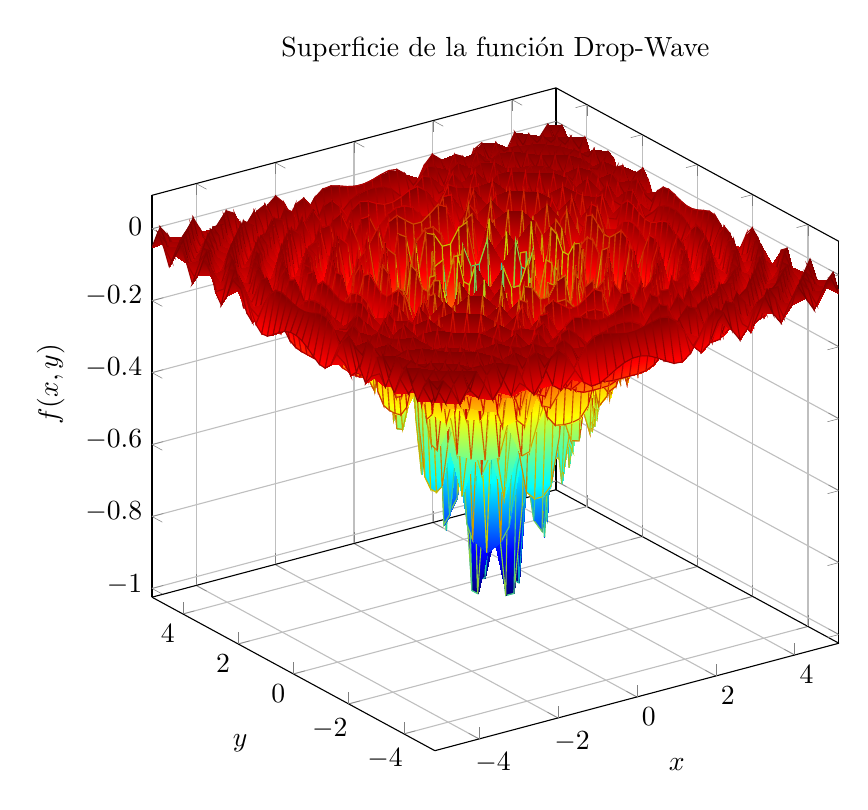
\begin{tikzpicture}
        \begin{axis}[
            title={Superficie de la función Drop-Wave},
            xlabel={$x$},
            ylabel={$y$},
            zlabel={$f(x,y)$},
            grid=major,
            colormap/jet,
            domain=-5.12:5.12,
            y domain=-5.12:5.12,
            samples=50,
            view={-35}{25},
            width=0.85\textwidth,
            height=10cm
        ]

        \addplot3[
            surf,
            shader=faceted interp
        ]
        {-(1 + cos(deg(12*sqrt(x^2 + y^2)))) / (0.5*(x^2 + y^2) + 2)};

        \end{axis}
    \end{tikzpicture}
    \caption*{Representación tridimensional de la función Drop-Wave.}
    \label{fig:drop_wave_3d}
\end{figure}

La función se define típicamente en dos dimensiones mediante la siguiente ecuación:
$$f(x) = -\frac{1 + \cos(12\sqrt{x_{1}^{2} + x_{2}^{2}})}{0.5(x_{1}^{2} + x_{2}^{2}) + 2}$$

% SUB-SECCIÓN
\subsection{Problema}

El problema central de este proyecto consiste en la optimización de la función Drop-Wave, la cual está catalogada como una función de prueba (benchmark) de tipo multimodal.
El objetivo principal es encontrar el punto donde esta función alcanza su valor mínimo posible dentro de un espacio de búsqueda determinado.

\subsubsection{Espacio de búsqueda y óptimo global}
Para delimitar el problema de optimización, se establecen las siguientes condiciones de frontera y metas teóricas:
\begin{itemize}
    \item \textbf{Espacio de Búsqueda:} El dominio para la evaluación de las soluciones está definido estrictamente en el intervalo continuo $x_{i} \in [-5.12, 5.12]$.
    \item \textbf{Mínimo Global:} El valor óptimo teórico que el algoritmo debe buscar alcanzar se localiza en el origen de las coordenadas, donde $f(0,0) = -1$.
\end{itemize}

\subsubsection{Naturaleza del desafío}
La dificultad principal que introduce la función Drop-Wave es la presencia de múltiples mínimos locales distribuidos en forma de ondas concéntricas alrededor del centro.
Esta característica topológica castiga fuertemente la falta de diversidad durante la búsqueda.

Si el método de optimización no posee el impulso suficiente para "saltar" las crestas de estas ondas (lo cual en los algoritmos genéticos se
logra mediante el operador de mutación), la población tiende a estancarse y converger prematuramente en los anillos exteriores, perdiendo la
capacidad de encontrar el pozo central en el origen.

% ------------------------------------------------------------------------------
% NUEVA SECCIÓN
% ------------------------------------------------------------------------------
\clearpage
\section{Planteamiento del problema}

% SUB-SECCIÓN
\subsection{Definición de un estado del problema}
En el contexto de la optimización de la función Drop-Wave, un estado $E$ representa un punto de evaluación específico sobre la superficie multidimensional de
la función; es decir, una posible solución al problema.

Matemáticamente, debido a la naturaleza de la función, un estado cualquiera se describe de manera precisa como un vector o 2-tupla de números reales:
$$E := (x_{1}, x_{2}) \text{ con } x_{i} \in \mathbb{R}$$

Cada componente $x_{i}$ de la tupla representa una coordenada espacial en el plano base sobre el cual se proyecta la superficie de la función. El problema parte
de un estado inicial (o múltiples estados iniciales) generados aleatoriamente, y el objetivo es encontrar un estado final $E_{f} = (0, 0)$ que, al ser evaluado,
resulte en el mínimo global teórico de $-1$.

\subsection{Representación de un estado para el algoritmo de optimización}
Dado que el método de solución se basa en algoritmos genéticos, cada estado $E$ funge como un individuo (o cromosoma) dentro de una población. Para asegurar la
compatibilidad con los operadores evolutivos en un dominio continuo, se adopta una representación mediante codificación real.

El espacio de búsqueda está conformado por todos los números reales comprendidos en el dominio delimitado por la función, es decir:
$$[-5.12, 5.12] \times [-5.12, 5.12]$$

La representación de $x_{1}$ y $x_{2}$ como números de punto flotante es fundamental para explorar activamente este espacio continuo, ya que permite la aplicación
directa de las siguientes operaciones genéticas:

\begin{itemize}
    \item \textbf{Operación de cruce:} La representación vectorial real permite realizar una recombinación aritmética, donde los genes de los padres se promedian o
        interpolan matemáticamente para producir descendientes viables dentro de los límites del espacio de búsqueda.

    \item \textbf{Operación de mutación:} Al ser números reales, la mutación se implementa mediante la inyección de ruido Gaussiano a los valores de $x_{1}$ o $x_{2}$.
        Esta alteración matemática es vital para que el individuo resultante logre "saltar" las múltiples crestas que caracterizan a la función Drop-Wave, proveyendo la
        diversidad necesaria para escapar de los mínimos locales concéntricos.
\end{itemize}

% ------------------------------------------------------------------------------
% NUEVA SECCIÓN
% ------------------------------------------------------------------------------

\clearpage
\section{Metodología}

Para abordar la optimización de la función Drop-Wave, se diseñó e implementó un Algoritmo Genético (AG) de codificación real. El proceso evolutivo opera sobre una
población constante de $100$ individuos a lo largo de $40$ generaciones. La estrategia para la transición de estados y la selección de nuevos individuos se divide
en los siguientes mecanismos iterativos:

\begin{itemize}
    \item \textbf{Inicialización y Evaluación:} La población inicial se distribuye aleatoriamente en el espacio de búsqueda continuo mediante una distribución uniforme
        iterada en el intervalo $[-5.12, 5.12]$. La calidad de cada individuo se cuantifica mediante una función de aptitud o \textit{fitness}. Dado que el objetivo es
        minimizar $f(x)$, la función de aptitud está diseñada para maximizar su negativo algebraico, es decir, $\Phi(x) = -f(x)$.

    \item \textbf{Elitismo:} Para asegurar una convergencia monótona y evitar la pérdida accidental de soluciones óptimas, se aplica un criterio de elitismo estricto.
        El individuo con la mayor aptitud de la generación actual pasa directamente y sin modificaciones a la siguiente generación.

    \item \textbf{Selección de progenitores:} La extracción de padres de la población se realiza mediante una selección por torneo con un tamaño de $k=3$. Se eligen aleatoriamente tres candidatos y el que posea el valor más alto en la función de aptitud gana el derecho a reproducirse, garantizando una presión selectiva constante.

    \item \textbf{Cruza (Recombinación):} Se aplica un cruce aritmético para explotar las regiones prometedoras del espacio. Por cada par de padres seleccionados,
        se genera un peso aleatorio $\alpha \in [0, 1]$. Los dos hijos resultantes son combinaciones lineales de los progenitores, asegurando que su ubicación permanezca
        dentro del dominio válido.
        $$\vec{h}_1 = \alpha \vec{p}_1 + (1 - \alpha)\vec{p}_2$$
        $$\vec{h}_2 = (1 - \alpha)\vec{p}_1 + \alpha \vec{p}_2$$

    \item \textbf{Mutación:} Para preservar la diversidad poblacional y otorgar a los individuos la capacidad de "saltar" los múltiples mínimos locales (crestas)
        de la función Drop-Wave, se emplea una mutación gaussiana. Cada gen (coordenada) tiene un $15\%$ de probabilidad de ser mutado. Si la mutación ocurre, se
        le añade un ruido aleatorio extraído de una distribución normal centrada en $0$ con una desviación estándar $\sigma = 0.5$. Posteriormente, se aplica un
        mecanismo de restricción (\textit{clipping}) para forzar que la nueva coordenada no exceda los límites de $\pm 5.12$.
\end{itemize}

% ------------------------------------------------------------------------------
% REFERENCIAS, revisar configuración \stylecitereferences
% ------------------------------------------------------------------------------
\clearpage
\nocite{*}
\bibliography{library}
